\chapter{Versuche in der Simulation}
\label{chap:versuche}



{\color{red}
    %\lstinputlisting[caption={Eine klassische \lstinline{main.m}-Datei aus Objective-C}]{chapter3/main.m}
    Ideen zu Fragestellungen die Versuche n�tig machen:
    \begin{itemize}
    \item Wie viele Bilder pro Zeit/Stecke sind n�tig? Wie genau will man dabei noch sein? Evtl. Bildfrequenz zu Mittlerer Unsicherheit Darstellen?
    \item Wie wirkt es sich aus, wenn teile des Musters verdeckt sind? Ist eine Lokalisation auch bei st�ndiger Verdeckung m�glich?
    \item Wie muss das Muster aufgebaut sein? Was f�r Fehler k�nne entstehen, wenn ein ungeeignetes Muster verwendet wird?
    \item Wie gut kommt der Filter mit Systematischen Fehlern zurecht?
    \end{itemize}
}

\section{Versuche zur Genauigkeit des Messmodells}
In einer ersten Versuchsreihe, soll die Genauigkeit des im Partikel Filter verwendeten Messmodells untersucht werden. Daf�r soll zu einem gegebenen Bild m�glichst der gesamte Zustandsraum mit dem in Kapitel \ref{subsec:messmodell} beschriebenen Verfahren bewertet werden. Je nach dem wie viele Punkte im Zustandsraum einen hohen Score erhalten, l�sst darauf schlie�en wie genau die Zuordnung zwischen Bild und Pose funktioniert. Im ersten Durchlauf soll erst mal grob der gesamte Raum abgesucht werden. Er soll einen �berblick geben, wo starke Antworten liegen, die dann in weiteren Durchl�ufen genauer abgetastet werden k�nnen.

\begin{figure}[p]
    \centering
    \vspace{-40pt}
    % GNUPLOT: LaTeX picture with Postscript
\begingroup
  \makeatletter
  \providecommand\color[2][]{%
    \GenericError{(gnuplot) \space\space\space\@spaces}{%
      Package color not loaded in conjunction with
      terminal option `colourtext'%
    }{See the gnuplot documentation for explanation.%
    }{Either use 'blacktext' in gnuplot or load the package
      color.sty in LaTeX.}%
    \renewcommand\color[2][]{}%
  }%
  \providecommand\includegraphics[2][]{%
    \GenericError{(gnuplot) \space\space\space\@spaces}{%
      Package graphicx or graphics not loaded%
    }{See the gnuplot documentation for explanation.%
    }{The gnuplot epslatex terminal needs graphicx.sty or graphics.sty.}%
    \renewcommand\includegraphics[2][]{}%
  }%
  \providecommand\rotatebox[2]{#2}%
  \@ifundefined{ifGPcolor}{%
    \newif\ifGPcolor
    \GPcolortrue
  }{}%
  \@ifundefined{ifGPblacktext}{%
    \newif\ifGPblacktext
    \GPblacktexttrue
  }{}%
  % define a \g@addto@macro without @ in the name:
  \let\gplgaddtomacro\g@addto@macro
  % define empty templates for all commands taking text:
  \gdef\gplbacktext{}%
  \gdef\gplfronttext{}%
  \makeatother
  \ifGPblacktext
    % no textcolor at all
    \def\colorrgb#1{}%
    \def\colorgray#1{}%
  \else
    % gray or color?
    \ifGPcolor
      \def\colorrgb#1{\color[rgb]{#1}}%
      \def\colorgray#1{\color[gray]{#1}}%
      \expandafter\def\csname LTw\endcsname{\color{white}}%
      \expandafter\def\csname LTb\endcsname{\color{black}}%
      \expandafter\def\csname LTa\endcsname{\color{black}}%
      \expandafter\def\csname LT0\endcsname{\color[rgb]{1,0,0}}%
      \expandafter\def\csname LT1\endcsname{\color[rgb]{0,1,0}}%
      \expandafter\def\csname LT2\endcsname{\color[rgb]{0,0,1}}%
      \expandafter\def\csname LT3\endcsname{\color[rgb]{1,0,1}}%
      \expandafter\def\csname LT4\endcsname{\color[rgb]{0,1,1}}%
      \expandafter\def\csname LT5\endcsname{\color[rgb]{1,1,0}}%
      \expandafter\def\csname LT6\endcsname{\color[rgb]{0,0,0}}%
      \expandafter\def\csname LT7\endcsname{\color[rgb]{1,0.3,0}}%
      \expandafter\def\csname LT8\endcsname{\color[rgb]{0.5,0.5,0.5}}%
    \else
      % gray
      \def\colorrgb#1{\color{black}}%
      \def\colorgray#1{\color[gray]{#1}}%
      \expandafter\def\csname LTw\endcsname{\color{white}}%
      \expandafter\def\csname LTb\endcsname{\color{black}}%
      \expandafter\def\csname LTa\endcsname{\color{black}}%
      \expandafter\def\csname LT0\endcsname{\color{black}}%
      \expandafter\def\csname LT1\endcsname{\color{black}}%
      \expandafter\def\csname LT2\endcsname{\color{black}}%
      \expandafter\def\csname LT3\endcsname{\color{black}}%
      \expandafter\def\csname LT4\endcsname{\color{black}}%
      \expandafter\def\csname LT5\endcsname{\color{black}}%
      \expandafter\def\csname LT6\endcsname{\color{black}}%
      \expandafter\def\csname LT7\endcsname{\color{black}}%
      \expandafter\def\csname LT8\endcsname{\color{black}}%
    \fi
  \fi
  \setlength{\unitlength}{0.0500bp}%
  \begin{picture}(8640.00,7200.00)%
    \gplgaddtomacro\gplbacktext{%
    }%
    \gplgaddtomacro\gplfronttext{%
      \csname LTb\endcsname%
      \put(5811,5663){\makebox(0,0)[r]{\strut{}     0.8}}%
      \csname LTb\endcsname%
      \put(5811,5443){\makebox(0,0)[r]{\strut{}     0.6}}%
      \csname LTb\endcsname%
      \put(5811,5223){\makebox(0,0)[r]{\strut{}     0.4}}%
      \csname LTb\endcsname%
      \put(5811,5003){\makebox(0,0)[r]{\strut{}     0.2}}%
      \csname LTb\endcsname%
      \put(2155,1078){\makebox(0,0){\strut{}-6}}%
      \csname LTb\endcsname%
      \put(4320,1078){\makebox(0,0){\strut{} 0}}%
      \csname LTb\endcsname%
      \put(6485,1078){\makebox(0,0){\strut{} 6}}%
      \put(4320,748){\makebox(0,0){\strut{}XAchse in Metern}}%
      \csname LTb\endcsname%
      \put(1802,1545){\makebox(0,0)[r]{\strut{}-6}}%
      \csname LTb\endcsname%
      \put(1802,3710){\makebox(0,0)[r]{\strut{} 0}}%
      \csname LTb\endcsname%
      \put(1802,5875){\makebox(0,0)[r]{\strut{} 6}}%
      \put(1472,3710){\rotatebox{-270}{\makebox(0,0){\strut{}YAchse in Metern}}}%
    }%
    \gplbacktext
    \put(0,0){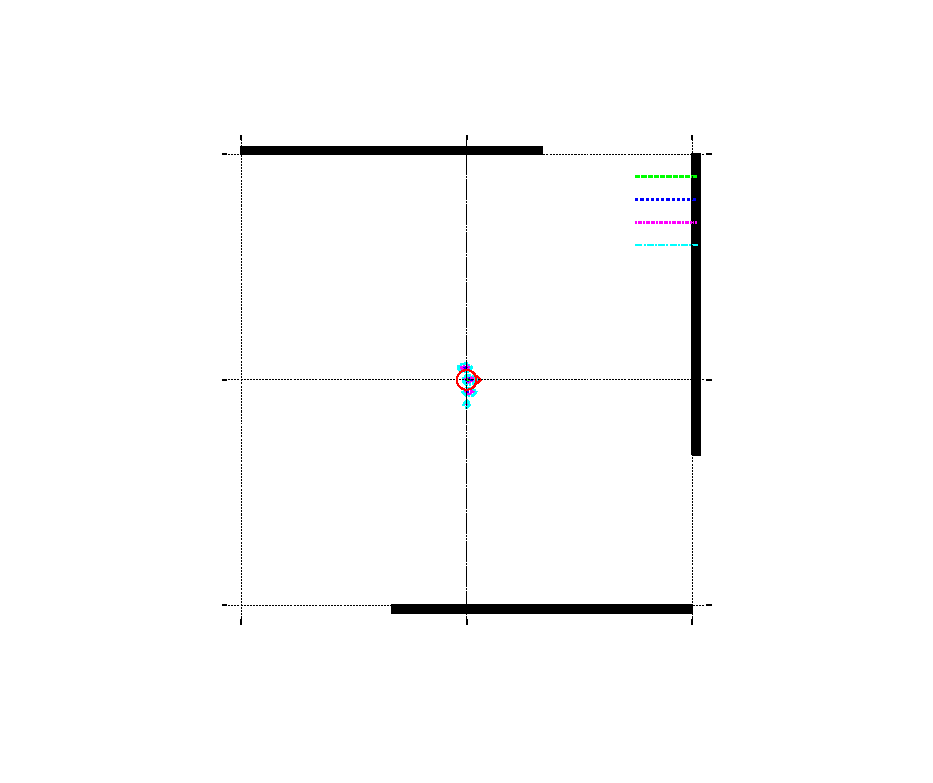
\includegraphics{chapter3/full_6x6_5cm_005Deg}}%
    \gplfronttext
  \end{picture}%
\endgroup

    \vspace{-20pt}
    % GNUPLOT: LaTeX picture with Postscript
\begingroup
  \makeatletter
  \providecommand\color[2][]{%
    \GenericError{(gnuplot) \space\space\space\@spaces}{%
      Package color not loaded in conjunction with
      terminal option `colourtext'%
    }{See the gnuplot documentation for explanation.%
    }{Either use 'blacktext' in gnuplot or load the package
      color.sty in LaTeX.}%
    \renewcommand\color[2][]{}%
  }%
  \providecommand\includegraphics[2][]{%
    \GenericError{(gnuplot) \space\space\space\@spaces}{%
      Package graphicx or graphics not loaded%
    }{See the gnuplot documentation for explanation.%
    }{The gnuplot epslatex terminal needs graphicx.sty or graphics.sty.}%
    \renewcommand\includegraphics[2][]{}%
  }%
  \providecommand\rotatebox[2]{#2}%
  \@ifundefined{ifGPcolor}{%
    \newif\ifGPcolor
    \GPcolortrue
  }{}%
  \@ifundefined{ifGPblacktext}{%
    \newif\ifGPblacktext
    \GPblacktexttrue
  }{}%
  % define a \g@addto@macro without @ in the name:
  \let\gplgaddtomacro\g@addto@macro
  % define empty templates for all commands taking text:
  \gdef\gplbacktext{}%
  \gdef\gplfronttext{}%
  \makeatother
  \ifGPblacktext
    % no textcolor at all
    \def\colorrgb#1{}%
    \def\colorgray#1{}%
  \else
    % gray or color?
    \ifGPcolor
      \def\colorrgb#1{\color[rgb]{#1}}%
      \def\colorgray#1{\color[gray]{#1}}%
      \expandafter\def\csname LTw\endcsname{\color{white}}%
      \expandafter\def\csname LTb\endcsname{\color{black}}%
      \expandafter\def\csname LTa\endcsname{\color{black}}%
      \expandafter\def\csname LT0\endcsname{\color[rgb]{1,0,0}}%
      \expandafter\def\csname LT1\endcsname{\color[rgb]{0,1,0}}%
      \expandafter\def\csname LT2\endcsname{\color[rgb]{0,0,1}}%
      \expandafter\def\csname LT3\endcsname{\color[rgb]{1,0,1}}%
      \expandafter\def\csname LT4\endcsname{\color[rgb]{0,1,1}}%
      \expandafter\def\csname LT5\endcsname{\color[rgb]{1,1,0}}%
      \expandafter\def\csname LT6\endcsname{\color[rgb]{0,0,0}}%
      \expandafter\def\csname LT7\endcsname{\color[rgb]{1,0.3,0}}%
      \expandafter\def\csname LT8\endcsname{\color[rgb]{0.5,0.5,0.5}}%
    \else
      % gray
      \def\colorrgb#1{\color{black}}%
      \def\colorgray#1{\color[gray]{#1}}%
      \expandafter\def\csname LTw\endcsname{\color{white}}%
      \expandafter\def\csname LTb\endcsname{\color{black}}%
      \expandafter\def\csname LTa\endcsname{\color{black}}%
      \expandafter\def\csname LT0\endcsname{\color{black}}%
      \expandafter\def\csname LT1\endcsname{\color{black}}%
      \expandafter\def\csname LT2\endcsname{\color{black}}%
      \expandafter\def\csname LT3\endcsname{\color{black}}%
      \expandafter\def\csname LT4\endcsname{\color{black}}%
      \expandafter\def\csname LT5\endcsname{\color{black}}%
      \expandafter\def\csname LT6\endcsname{\color{black}}%
      \expandafter\def\csname LT7\endcsname{\color{black}}%
      \expandafter\def\csname LT8\endcsname{\color{black}}%
    \fi
  \fi
  \setlength{\unitlength}{0.0500bp}%
  \begin{picture}(8640.00,7200.00)%
    \gplgaddtomacro\gplbacktext{%
    }%
    \gplgaddtomacro\gplfronttext{%
      \csname LTb\endcsname%
      \put(5811,5663){\makebox(0,0)[r]{\strut{}       3}}%
      \csname LTb\endcsname%
      \put(5811,5443){\makebox(0,0)[r]{\strut{}       2}}%
      \csname LTb\endcsname%
      \put(5811,5223){\makebox(0,0)[r]{\strut{}       1}}%
      \csname LTb\endcsname%
      \put(1974,1078){\makebox(0,0){\strut{}-1}}%
      \csname LTb\endcsname%
      \put(4320,1078){\makebox(0,0){\strut{} 0}}%
      \csname LTb\endcsname%
      \put(6666,1078){\makebox(0,0){\strut{} 1}}%
      \put(4320,748){\makebox(0,0){\strut{}XAchse in Metern}}%
      \csname LTb\endcsname%
      \put(1802,1364){\makebox(0,0)[r]{\strut{}-1}}%
      \csname LTb\endcsname%
      \put(1802,3710){\makebox(0,0)[r]{\strut{} 0}}%
      \csname LTb\endcsname%
      \put(1802,6056){\makebox(0,0)[r]{\strut{} 1}}%
      \put(1472,3710){\rotatebox{-270}{\makebox(0,0){\strut{}YAchse in Metern}}}%
    }%
    \gplbacktext
    \put(0,0){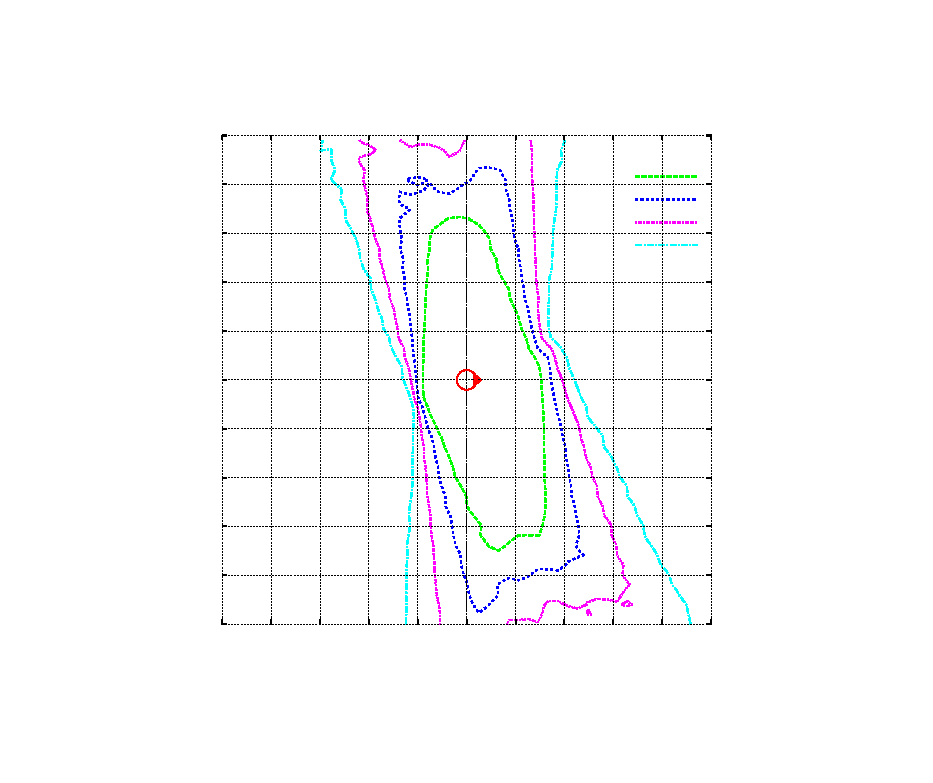
\includegraphics{chapter3/position_variance_on_picture}}%
    \gplfronttext
  \end{picture}%
\endgroup

    \caption{Antwort des Messmodells zu einem Bild an der rot markierten Position oben: 5cm Raster 3� Schritte unten: 1cm Raster 0.3� Schritte}
    \label{fig:messmodellPos}
\end{figure}

F�r die Versuchsreihe wird der Zustandsraum zun�chst grob in 5~cm Rasterschritten durchsucht. Dabei wird die Orientierung in 0,05 Rad (2,86�) Schritte Aufgeteilt. In drei Schleifen wird so der Zustandsraum durchlaufen. Als Messung wurde ein am Ursprung (x = 0, y = 0, psi = 0) aufgenommenes Bild verwendet. F�r die Darstellung in Abbildung \ref{fig:messmodellPos} oben, wurden H�henlinien der Messantwort geplottet. Dabei wurde jeweils nur die st�rkste Antwort an einer Position �ber alle Winkel gew�hlt. Bei einem Zweiten Durchlauf wurde die Positionsrasterung auf 1~cm Schritte, und die Winkelschritte auf 0,005 Rad (0.28�) verkleinert. Zu sehen ist dies auf Abbildung \ref{fig:messmodellPos} unten. Um den Einfluss des Winkels darzustellen wurde in Abbildung \ref{fig:messmodellAngle} die Antwort entlang einer Linie mit $x=0.0$ geplottet. 

\begin{figure}[h]
    \centering
    % GNUPLOT: LaTeX picture with Postscript
\begingroup
  \makeatletter
  \providecommand\color[2][]{%
    \GenericError{(gnuplot) \space\space\space\@spaces}{%
      Package color not loaded in conjunction with
      terminal option `colourtext'%
    }{See the gnuplot documentation for explanation.%
    }{Either use 'blacktext' in gnuplot or load the package
      color.sty in LaTeX.}%
    \renewcommand\color[2][]{}%
  }%
  \providecommand\includegraphics[2][]{%
    \GenericError{(gnuplot) \space\space\space\@spaces}{%
      Package graphicx or graphics not loaded%
    }{See the gnuplot documentation for explanation.%
    }{The gnuplot epslatex terminal needs graphicx.sty or graphics.sty.}%
    \renewcommand\includegraphics[2][]{}%
  }%
  \providecommand\rotatebox[2]{#2}%
  \@ifundefined{ifGPcolor}{%
    \newif\ifGPcolor
    \GPcolortrue
  }{}%
  \@ifundefined{ifGPblacktext}{%
    \newif\ifGPblacktext
    \GPblacktexttrue
  }{}%
  % define a \g@addto@macro without @ in the name:
  \let\gplgaddtomacro\g@addto@macro
  % define empty templates for all commands taking text:
  \gdef\gplbacktext{}%
  \gdef\gplfronttext{}%
  \makeatother
  \ifGPblacktext
    % no textcolor at all
    \def\colorrgb#1{}%
    \def\colorgray#1{}%
  \else
    % gray or color?
    \ifGPcolor
      \def\colorrgb#1{\color[rgb]{#1}}%
      \def\colorgray#1{\color[gray]{#1}}%
      \expandafter\def\csname LTw\endcsname{\color{white}}%
      \expandafter\def\csname LTb\endcsname{\color{black}}%
      \expandafter\def\csname LTa\endcsname{\color{black}}%
      \expandafter\def\csname LT0\endcsname{\color[rgb]{1,0,0}}%
      \expandafter\def\csname LT1\endcsname{\color[rgb]{0,1,0}}%
      \expandafter\def\csname LT2\endcsname{\color[rgb]{0,0,1}}%
      \expandafter\def\csname LT3\endcsname{\color[rgb]{1,0,1}}%
      \expandafter\def\csname LT4\endcsname{\color[rgb]{0,1,1}}%
      \expandafter\def\csname LT5\endcsname{\color[rgb]{1,1,0}}%
      \expandafter\def\csname LT6\endcsname{\color[rgb]{0,0,0}}%
      \expandafter\def\csname LT7\endcsname{\color[rgb]{1,0.3,0}}%
      \expandafter\def\csname LT8\endcsname{\color[rgb]{0.5,0.5,0.5}}%
    \else
      % gray
      \def\colorrgb#1{\color{black}}%
      \def\colorgray#1{\color[gray]{#1}}%
      \expandafter\def\csname LTw\endcsname{\color{white}}%
      \expandafter\def\csname LTb\endcsname{\color{black}}%
      \expandafter\def\csname LTa\endcsname{\color{black}}%
      \expandafter\def\csname LT0\endcsname{\color{black}}%
      \expandafter\def\csname LT1\endcsname{\color{black}}%
      \expandafter\def\csname LT2\endcsname{\color{black}}%
      \expandafter\def\csname LT3\endcsname{\color{black}}%
      \expandafter\def\csname LT4\endcsname{\color{black}}%
      \expandafter\def\csname LT5\endcsname{\color{black}}%
      \expandafter\def\csname LT6\endcsname{\color{black}}%
      \expandafter\def\csname LT7\endcsname{\color{black}}%
      \expandafter\def\csname LT8\endcsname{\color{black}}%
    \fi
  \fi
  \setlength{\unitlength}{0.0500bp}%
  \begin{picture}(8640.00,7200.00)%
    \gplgaddtomacro\gplbacktext{%
    }%
    \gplgaddtomacro\gplfronttext{%
      \csname LTb\endcsname%
      \put(5811,5663){\makebox(0,0)[r]{\strut{}     0.8}}%
      \csname LTb\endcsname%
      \put(5811,5443){\makebox(0,0)[r]{\strut{}     0.6}}%
      \csname LTb\endcsname%
      \put(5811,5223){\makebox(0,0)[r]{\strut{}     0.4}}%
      \csname LTb\endcsname%
      \put(5811,5003){\makebox(0,0)[r]{\strut{}     0.2}}%
      \csname LTb\endcsname%
      \put(1974,1078){\makebox(0,0){\strut{}-6}}%
      \csname LTb\endcsname%
      \put(2365,1078){\makebox(0,0){\strut{}-5}}%
      \csname LTb\endcsname%
      \put(2756,1078){\makebox(0,0){\strut{}-4}}%
      \csname LTb\endcsname%
      \put(3147,1078){\makebox(0,0){\strut{}-3}}%
      \csname LTb\endcsname%
      \put(3538,1078){\makebox(0,0){\strut{}-2}}%
      \csname LTb\endcsname%
      \put(3929,1078){\makebox(0,0){\strut{}-1}}%
      \csname LTb\endcsname%
      \put(4320,1078){\makebox(0,0){\strut{} 0}}%
      \csname LTb\endcsname%
      \put(4711,1078){\makebox(0,0){\strut{} 1}}%
      \csname LTb\endcsname%
      \put(5102,1078){\makebox(0,0){\strut{} 2}}%
      \csname LTb\endcsname%
      \put(5493,1078){\makebox(0,0){\strut{} 3}}%
      \csname LTb\endcsname%
      \put(5884,1078){\makebox(0,0){\strut{} 4}}%
      \csname LTb\endcsname%
      \put(6275,1078){\makebox(0,0){\strut{} 5}}%
      \csname LTb\endcsname%
      \put(6666,1078){\makebox(0,0){\strut{} 6}}%
      \put(4320,748){\makebox(0,0){\strut{}XAchse Winkel in Grad}}%
      \csname LTb\endcsname%
      \put(1802,1364){\makebox(0,0)[r]{\strut{}-0.5}}%
      \csname LTb\endcsname%
      \put(1802,1833){\makebox(0,0)[r]{\strut{}-0.4}}%
      \csname LTb\endcsname%
      \put(1802,2303){\makebox(0,0)[r]{\strut{}-0.3}}%
      \csname LTb\endcsname%
      \put(1802,2772){\makebox(0,0)[r]{\strut{}-0.2}}%
      \csname LTb\endcsname%
      \put(1802,3241){\makebox(0,0)[r]{\strut{}-0.1}}%
      \csname LTb\endcsname%
      \put(1802,3710){\makebox(0,0)[r]{\strut{} 0}}%
      \csname LTb\endcsname%
      \put(1802,4179){\makebox(0,0)[r]{\strut{} 0.1}}%
      \csname LTb\endcsname%
      \put(1802,4648){\makebox(0,0)[r]{\strut{} 0.2}}%
      \csname LTb\endcsname%
      \put(1802,5117){\makebox(0,0)[r]{\strut{} 0.3}}%
      \csname LTb\endcsname%
      \put(1802,5587){\makebox(0,0)[r]{\strut{} 0.4}}%
      \csname LTb\endcsname%
      \put(1802,6056){\makebox(0,0)[r]{\strut{} 0.5}}%
      \put(1208,3710){\rotatebox{-270}{\makebox(0,0){\strut{}YAchse in Metern}}}%
    }%
    \gplbacktext
    \put(0,0){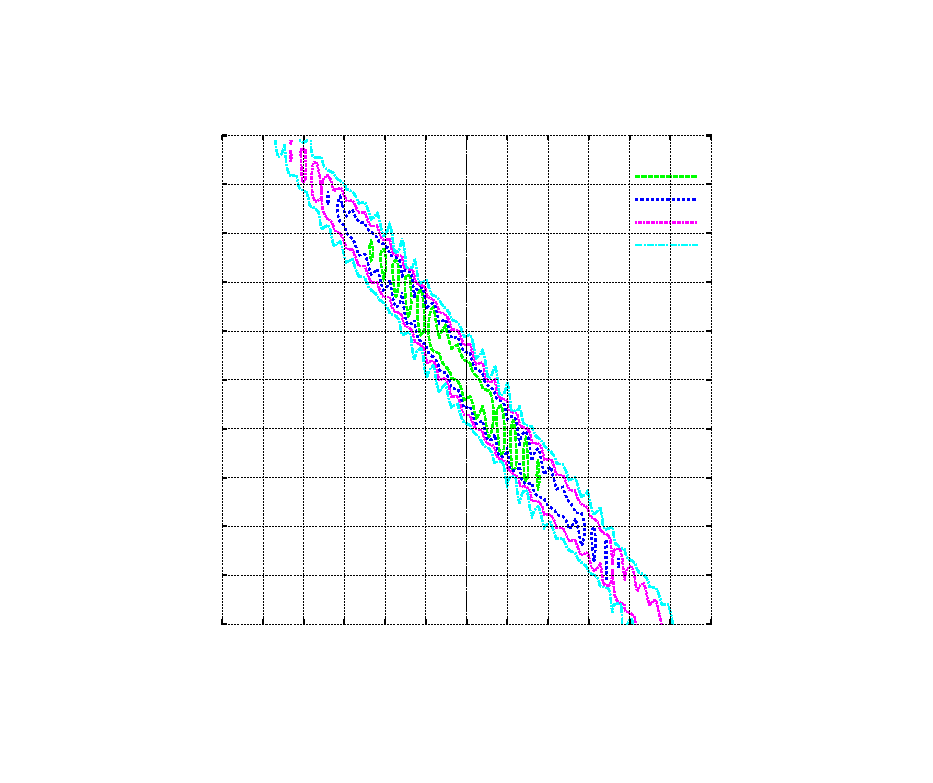
\includegraphics{chapter3/pTOyANDangle_1cm_0005Deg_xIS0}}%
    \gplfronttext
  \end{picture}%
\endgroup

    \caption{Antwort des Messmodells bei x=0.0}
    \label{fig:messmodellAngle}
\end{figure}

In Abbildung \ref{fig:messmodellPos} oben, kann man sehen, das die Antwort des Messmodells nur um die erwartete Position sichtbar einen hohen Score ergibt. Darunter sieht man einen Vergr��erten Ausschnitt. Hier f�llt auf, dass die H�ufung sich leicht schr�g liegt. Dies liegt vermutlich daran, dass die Lichtwand auf der das Muster abgebildet ist, nicht zentral vor dem Roboter steht, sondern in Y-Richtung verschoben ist. Die H�ufung der Antworten streut vor allem entlang der Y-Achse. Also bei einer seitlichen Verschiebung des Roboters. Dabei sind innerhalb von $\pm 30\ cm$ immer noch Scores oberhalb von 0,8 m�glich. Entlang der X-Achse ist eine Streuung zwischen $+15$ und $-10$~cm zu erkennen. Durch die H�henlinien sieht man, dass entlang der x-Achse der Score eine gro�e Steigung hat. Dies f�hrt zu einer relativ scharfen Kante in der in dieser Richtung. Auf der y-Achse dagegen, ist die Steigung schw�che und bildet keine so scharfe Kante. Aus Abbildung \ref{fig:messmodellAngle} l�sst sich entnehmen, dass bei einer Verschiebung entlang der Y-Achse eine Drehung des Roboters n�tig ist, um eine Pose zu erhalten die einen guten Score erh�lt.  
\section{Versuche zur Bildaufnahmefrequenz}
Es soll untersucht werden in welchen Intervallen Bilder ben�tigt werden. Wie stark der Einfluss der Fahrkurve darauf ist, und welche Faktoren die Bildaufnahmefrequenz beeinflussen k�nnen.
\begin{figure}[p]
    \centering
    \vspace{-30pt}
    % GNUPLOT: LaTeX picture with Postscript
\begingroup
  \makeatletter
  \providecommand\color[2][]{%
    \GenericError{(gnuplot) \space\space\space\@spaces}{%
      Package color not loaded in conjunction with
      terminal option `colourtext'%
    }{See the gnuplot documentation for explanation.%
    }{Either use 'blacktext' in gnuplot or load the package
      color.sty in LaTeX.}%
    \renewcommand\color[2][]{}%
  }%
  \providecommand\includegraphics[2][]{%
    \GenericError{(gnuplot) \space\space\space\@spaces}{%
      Package graphicx or graphics not loaded%
    }{See the gnuplot documentation for explanation.%
    }{The gnuplot epslatex terminal needs graphicx.sty or graphics.sty.}%
    \renewcommand\includegraphics[2][]{}%
  }%
  \providecommand\rotatebox[2]{#2}%
  \@ifundefined{ifGPcolor}{%
    \newif\ifGPcolor
    \GPcolortrue
  }{}%
  \@ifundefined{ifGPblacktext}{%
    \newif\ifGPblacktext
    \GPblacktexttrue
  }{}%
  % define a \g@addto@macro without @ in the name:
  \let\gplgaddtomacro\g@addto@macro
  % define empty templates for all commands taking text:
  \gdef\gplbacktext{}%
  \gdef\gplfronttext{}%
  \makeatother
  \ifGPblacktext
    % no textcolor at all
    \def\colorrgb#1{}%
    \def\colorgray#1{}%
  \else
    % gray or color?
    \ifGPcolor
      \def\colorrgb#1{\color[rgb]{#1}}%
      \def\colorgray#1{\color[gray]{#1}}%
      \expandafter\def\csname LTw\endcsname{\color{white}}%
      \expandafter\def\csname LTb\endcsname{\color{black}}%
      \expandafter\def\csname LTa\endcsname{\color{black}}%
      \expandafter\def\csname LT0\endcsname{\color[rgb]{1,0,0}}%
      \expandafter\def\csname LT1\endcsname{\color[rgb]{0,1,0}}%
      \expandafter\def\csname LT2\endcsname{\color[rgb]{0,0,1}}%
      \expandafter\def\csname LT3\endcsname{\color[rgb]{1,0,1}}%
      \expandafter\def\csname LT4\endcsname{\color[rgb]{0,1,1}}%
      \expandafter\def\csname LT5\endcsname{\color[rgb]{1,1,0}}%
      \expandafter\def\csname LT6\endcsname{\color[rgb]{0,0,0}}%
      \expandafter\def\csname LT7\endcsname{\color[rgb]{1,0.3,0}}%
      \expandafter\def\csname LT8\endcsname{\color[rgb]{0.5,0.5,0.5}}%
    \else
      % gray
      \def\colorrgb#1{\color{black}}%
      \def\colorgray#1{\color[gray]{#1}}%
      \expandafter\def\csname LTw\endcsname{\color{white}}%
      \expandafter\def\csname LTb\endcsname{\color{black}}%
      \expandafter\def\csname LTa\endcsname{\color{black}}%
      \expandafter\def\csname LT0\endcsname{\color{black}}%
      \expandafter\def\csname LT1\endcsname{\color{black}}%
      \expandafter\def\csname LT2\endcsname{\color{black}}%
      \expandafter\def\csname LT3\endcsname{\color{black}}%
      \expandafter\def\csname LT4\endcsname{\color{black}}%
      \expandafter\def\csname LT5\endcsname{\color{black}}%
      \expandafter\def\csname LT6\endcsname{\color{black}}%
      \expandafter\def\csname LT7\endcsname{\color{black}}%
      \expandafter\def\csname LT8\endcsname{\color{black}}%
    \fi
  \fi
  \setlength{\unitlength}{0.0500bp}%
  \begin{picture}(5760.00,7200.00)%
    \gplgaddtomacro\gplbacktext{%
      \csname LTb\endcsname%
      \put(682,3005){\makebox(0,0)[r]{\strut{}-6}}%
      \csname LTb\endcsname%
      \put(682,4370){\makebox(0,0)[r]{\strut{} 0}}%
      \csname LTb\endcsname%
      \put(682,5734){\makebox(0,0)[r]{\strut{} 6}}%
      \csname LTb\endcsname%
      \put(1724,1875){\makebox(0,0){\strut{}-6}}%
      \csname LTb\endcsname%
      \put(3089,1875){\makebox(0,0){\strut{} 0}}%
      \csname LTb\endcsname%
      \put(4453,1875){\makebox(0,0){\strut{} 6}}%
      \csname LTb\endcsname%
      \put(176,4369){\rotatebox{-270}{\makebox(0,0){\strut{}Y-Achse in Metern}}}%
      \put(3088,1545){\makebox(0,0){\strut{}X-Achse in Metern}}%
    }%
    \gplgaddtomacro\gplfronttext{%
      \csname LTb\endcsname%
      \put(4245,833){\makebox(0,0)[r]{\strut{}$3\sigma$}}%
      \csname LTb\endcsname%
      \put(4245,613){\makebox(0,0)[r]{\strut{}Trajektorie des Roboters}}%
      \csname LTb\endcsname%
      \put(4245,393){\makebox(0,0)[r]{\strut{}Filter Sch�tzung}}%
      \csname LTb\endcsname%
      \put(4245,173){\makebox(0,0)[r]{\strut{}Update}}%
    }%
    \gplbacktext
    \put(0,0){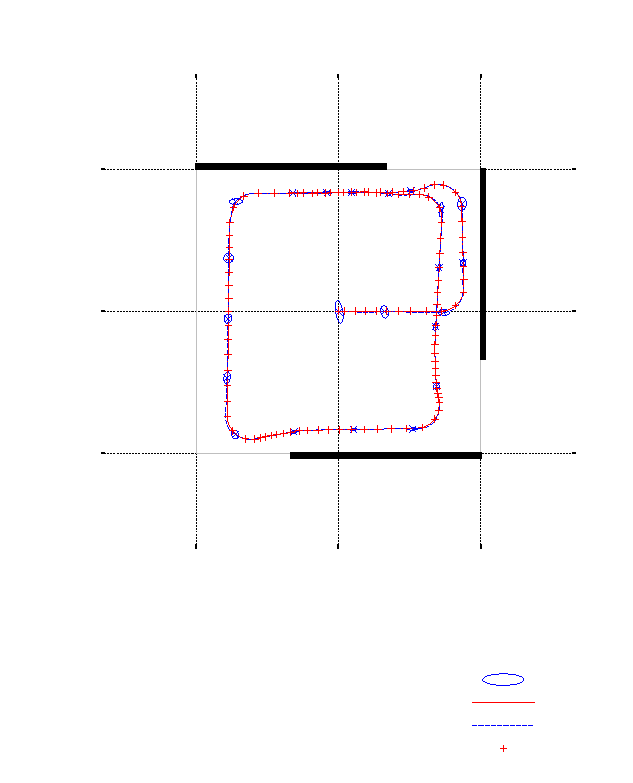
\includegraphics{chapter3/every500mspics}}%
    \gplfronttext
  \end{picture}%
\endgroup

    \vspace{-10pt}
    % GNUPLOT: LaTeX picture with Postscript
\begingroup
  \makeatletter
  \providecommand\color[2][]{%
    \GenericError{(gnuplot) \space\space\space\@spaces}{%
      Package color not loaded in conjunction with
      terminal option `colourtext'%
    }{See the gnuplot documentation for explanation.%
    }{Either use 'blacktext' in gnuplot or load the package
      color.sty in LaTeX.}%
    \renewcommand\color[2][]{}%
  }%
  \providecommand\includegraphics[2][]{%
    \GenericError{(gnuplot) \space\space\space\@spaces}{%
      Package graphicx or graphics not loaded%
    }{See the gnuplot documentation for explanation.%
    }{The gnuplot epslatex terminal needs graphicx.sty or graphics.sty.}%
    \renewcommand\includegraphics[2][]{}%
  }%
  \providecommand\rotatebox[2]{#2}%
  \@ifundefined{ifGPcolor}{%
    \newif\ifGPcolor
    \GPcolortrue
  }{}%
  \@ifundefined{ifGPblacktext}{%
    \newif\ifGPblacktext
    \GPblacktexttrue
  }{}%
  % define a \g@addto@macro without @ in the name:
  \let\gplgaddtomacro\g@addto@macro
  % define empty templates for all commands taking text:
  \gdef\gplbacktext{}%
  \gdef\gplfronttext{}%
  \makeatother
  \ifGPblacktext
    % no textcolor at all
    \def\colorrgb#1{}%
    \def\colorgray#1{}%
  \else
    % gray or color?
    \ifGPcolor
      \def\colorrgb#1{\color[rgb]{#1}}%
      \def\colorgray#1{\color[gray]{#1}}%
      \expandafter\def\csname LTw\endcsname{\color{white}}%
      \expandafter\def\csname LTb\endcsname{\color{black}}%
      \expandafter\def\csname LTa\endcsname{\color{black}}%
      \expandafter\def\csname LT0\endcsname{\color[rgb]{1,0,0}}%
      \expandafter\def\csname LT1\endcsname{\color[rgb]{0,1,0}}%
      \expandafter\def\csname LT2\endcsname{\color[rgb]{0,0,1}}%
      \expandafter\def\csname LT3\endcsname{\color[rgb]{1,0,1}}%
      \expandafter\def\csname LT4\endcsname{\color[rgb]{0,1,1}}%
      \expandafter\def\csname LT5\endcsname{\color[rgb]{1,1,0}}%
      \expandafter\def\csname LT6\endcsname{\color[rgb]{0,0,0}}%
      \expandafter\def\csname LT7\endcsname{\color[rgb]{1,0.3,0}}%
      \expandafter\def\csname LT8\endcsname{\color[rgb]{0.5,0.5,0.5}}%
    \else
      % gray
      \def\colorrgb#1{\color{black}}%
      \def\colorgray#1{\color[gray]{#1}}%
      \expandafter\def\csname LTw\endcsname{\color{white}}%
      \expandafter\def\csname LTb\endcsname{\color{black}}%
      \expandafter\def\csname LTa\endcsname{\color{black}}%
      \expandafter\def\csname LT0\endcsname{\color{black}}%
      \expandafter\def\csname LT1\endcsname{\color{black}}%
      \expandafter\def\csname LT2\endcsname{\color{black}}%
      \expandafter\def\csname LT3\endcsname{\color{black}}%
      \expandafter\def\csname LT4\endcsname{\color{black}}%
      \expandafter\def\csname LT5\endcsname{\color{black}}%
      \expandafter\def\csname LT6\endcsname{\color{black}}%
      \expandafter\def\csname LT7\endcsname{\color{black}}%
      \expandafter\def\csname LT8\endcsname{\color{black}}%
    \fi
  \fi
  \setlength{\unitlength}{0.0500bp}%
  \begin{picture}(5760.00,7200.00)%
    \gplgaddtomacro\gplbacktext{%
      \csname LTb\endcsname%
      \put(682,3005){\makebox(0,0)[r]{\strut{}-6}}%
      \csname LTb\endcsname%
      \put(682,4370){\makebox(0,0)[r]{\strut{} 0}}%
      \csname LTb\endcsname%
      \put(682,5734){\makebox(0,0)[r]{\strut{} 6}}%
      \csname LTb\endcsname%
      \put(1724,1875){\makebox(0,0){\strut{}-6}}%
      \csname LTb\endcsname%
      \put(3089,1875){\makebox(0,0){\strut{} 0}}%
      \csname LTb\endcsname%
      \put(4453,1875){\makebox(0,0){\strut{} 6}}%
      \csname LTb\endcsname%
      \put(176,4369){\rotatebox{-270}{\makebox(0,0){\strut{}Y-Achse in Metern}}}%
      \put(3088,1545){\makebox(0,0){\strut{}X-Achse in Metern}}%
    }%
    \gplgaddtomacro\gplfronttext{%
      \csname LTb\endcsname%
      \put(4245,833){\makebox(0,0)[r]{\strut{}$3\sigma$}}%
      \csname LTb\endcsname%
      \put(4245,613){\makebox(0,0)[r]{\strut{}Trajektorie des Roboters}}%
      \csname LTb\endcsname%
      \put(4245,393){\makebox(0,0)[r]{\strut{}Filter Sch�tzung}}%
      \csname LTb\endcsname%
      \put(4245,173){\makebox(0,0)[r]{\strut{}Update}}%
    }%
    \gplbacktext
    \put(0,0){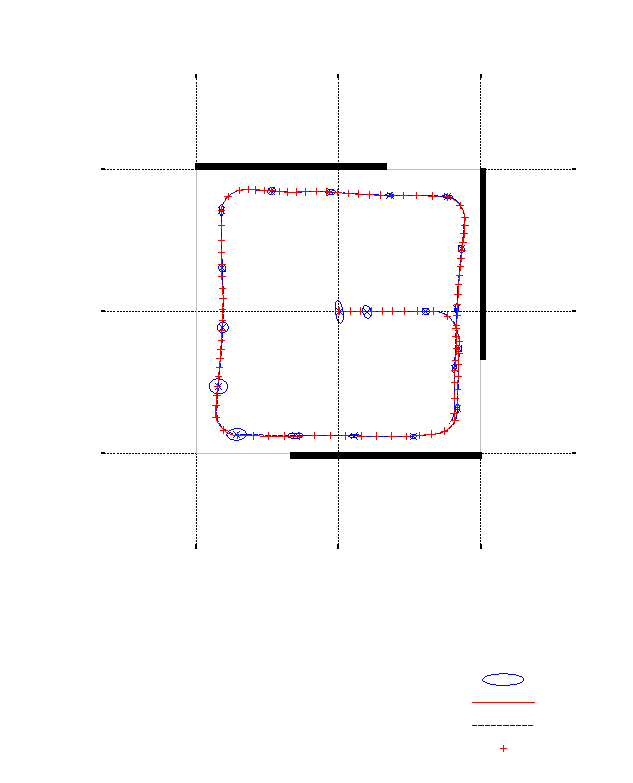
\includegraphics{chapter3/every500mspics_Loop_Clockwise}}%
    \gplfronttext
  \end{picture}%
\endgroup

    \caption{Fahrkurven oben gegen, und unten im Uhrzeigersinn}
    \label{every1000mspics}
\end{figure}
\begin{figure}[p]
    \centering
    \vspace{-30pt}
    % GNUPLOT: LaTeX picture with Postscript
\begingroup
  \makeatletter
  \providecommand\color[2][]{%
    \GenericError{(gnuplot) \space\space\space\@spaces}{%
      Package color not loaded in conjunction with
      terminal option `colourtext'%
    }{See the gnuplot documentation for explanation.%
    }{Either use 'blacktext' in gnuplot or load the package
      color.sty in LaTeX.}%
    \renewcommand\color[2][]{}%
  }%
  \providecommand\includegraphics[2][]{%
    \GenericError{(gnuplot) \space\space\space\@spaces}{%
      Package graphicx or graphics not loaded%
    }{See the gnuplot documentation for explanation.%
    }{The gnuplot epslatex terminal needs graphicx.sty or graphics.sty.}%
    \renewcommand\includegraphics[2][]{}%
  }%
  \providecommand\rotatebox[2]{#2}%
  \@ifundefined{ifGPcolor}{%
    \newif\ifGPcolor
    \GPcolortrue
  }{}%
  \@ifundefined{ifGPblacktext}{%
    \newif\ifGPblacktext
    \GPblacktexttrue
  }{}%
  % define a \g@addto@macro without @ in the name:
  \let\gplgaddtomacro\g@addto@macro
  % define empty templates for all commands taking text:
  \gdef\gplbacktext{}%
  \gdef\gplfronttext{}%
  \makeatother
  \ifGPblacktext
    % no textcolor at all
    \def\colorrgb#1{}%
    \def\colorgray#1{}%
  \else
    % gray or color?
    \ifGPcolor
      \def\colorrgb#1{\color[rgb]{#1}}%
      \def\colorgray#1{\color[gray]{#1}}%
      \expandafter\def\csname LTw\endcsname{\color{white}}%
      \expandafter\def\csname LTb\endcsname{\color{black}}%
      \expandafter\def\csname LTa\endcsname{\color{black}}%
      \expandafter\def\csname LT0\endcsname{\color[rgb]{1,0,0}}%
      \expandafter\def\csname LT1\endcsname{\color[rgb]{0,1,0}}%
      \expandafter\def\csname LT2\endcsname{\color[rgb]{0,0,1}}%
      \expandafter\def\csname LT3\endcsname{\color[rgb]{1,0,1}}%
      \expandafter\def\csname LT4\endcsname{\color[rgb]{0,1,1}}%
      \expandafter\def\csname LT5\endcsname{\color[rgb]{1,1,0}}%
      \expandafter\def\csname LT6\endcsname{\color[rgb]{0,0,0}}%
      \expandafter\def\csname LT7\endcsname{\color[rgb]{1,0.3,0}}%
      \expandafter\def\csname LT8\endcsname{\color[rgb]{0.5,0.5,0.5}}%
    \else
      % gray
      \def\colorrgb#1{\color{black}}%
      \def\colorgray#1{\color[gray]{#1}}%
      \expandafter\def\csname LTw\endcsname{\color{white}}%
      \expandafter\def\csname LTb\endcsname{\color{black}}%
      \expandafter\def\csname LTa\endcsname{\color{black}}%
      \expandafter\def\csname LT0\endcsname{\color{black}}%
      \expandafter\def\csname LT1\endcsname{\color{black}}%
      \expandafter\def\csname LT2\endcsname{\color{black}}%
      \expandafter\def\csname LT3\endcsname{\color{black}}%
      \expandafter\def\csname LT4\endcsname{\color{black}}%
      \expandafter\def\csname LT5\endcsname{\color{black}}%
      \expandafter\def\csname LT6\endcsname{\color{black}}%
      \expandafter\def\csname LT7\endcsname{\color{black}}%
      \expandafter\def\csname LT8\endcsname{\color{black}}%
    \fi
  \fi
  \setlength{\unitlength}{0.0500bp}%
  \begin{picture}(5760.00,7200.00)%
    \gplgaddtomacro\gplbacktext{%
      \csname LTb\endcsname%
      \put(682,3005){\makebox(0,0)[r]{\strut{}-6}}%
      \csname LTb\endcsname%
      \put(682,4369){\makebox(0,0)[r]{\strut{} 0}}%
      \csname LTb\endcsname%
      \put(682,5734){\makebox(0,0)[r]{\strut{} 6}}%
      \csname LTb\endcsname%
      \put(1724,1875){\makebox(0,0){\strut{}-6}}%
      \csname LTb\endcsname%
      \put(3088,1875){\makebox(0,0){\strut{} 0}}%
      \csname LTb\endcsname%
      \put(4453,1875){\makebox(0,0){\strut{} 6}}%
      \csname LTb\endcsname%
      \put(176,4369){\rotatebox{-270}{\makebox(0,0){\strut{}Y-Achse in Metern}}}%
      \put(3088,1545){\makebox(0,0){\strut{}X-Achse in Metern}}%
    }%
    \gplgaddtomacro\gplfronttext{%
      \csname LTb\endcsname%
      \put(4245,833){\makebox(0,0)[r]{\strut{}$3\sigma$}}%
      \csname LTb\endcsname%
      \put(4245,613){\makebox(0,0)[r]{\strut{}Trajektorie des Roboters}}%
      \csname LTb\endcsname%
      \put(4245,393){\makebox(0,0)[r]{\strut{}Filter Sch�tzung}}%
      \csname LTb\endcsname%
      \put(4245,173){\makebox(0,0)[r]{\strut{}Update}}%
    }%
    \gplbacktext
    \put(0,0){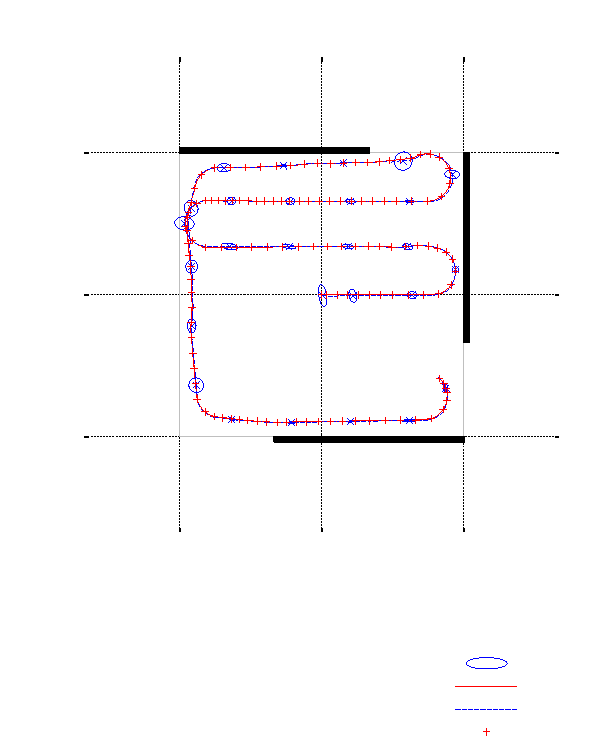
\includegraphics{chapter3/every500mspics_serpentinen}}%
    \gplfronttext
  \end{picture}%
\endgroup

    \vspace{-10pt}
    % GNUPLOT: LaTeX picture with Postscript
\begingroup
  \makeatletter
  \providecommand\color[2][]{%
    \GenericError{(gnuplot) \space\space\space\@spaces}{%
      Package color not loaded in conjunction with
      terminal option `colourtext'%
    }{See the gnuplot documentation for explanation.%
    }{Either use 'blacktext' in gnuplot or load the package
      color.sty in LaTeX.}%
    \renewcommand\color[2][]{}%
  }%
  \providecommand\includegraphics[2][]{%
    \GenericError{(gnuplot) \space\space\space\@spaces}{%
      Package graphicx or graphics not loaded%
    }{See the gnuplot documentation for explanation.%
    }{The gnuplot epslatex terminal needs graphicx.sty or graphics.sty.}%
    \renewcommand\includegraphics[2][]{}%
  }%
  \providecommand\rotatebox[2]{#2}%
  \@ifundefined{ifGPcolor}{%
    \newif\ifGPcolor
    \GPcolortrue
  }{}%
  \@ifundefined{ifGPblacktext}{%
    \newif\ifGPblacktext
    \GPblacktexttrue
  }{}%
  % define a \g@addto@macro without @ in the name:
  \let\gplgaddtomacro\g@addto@macro
  % define empty templates for all commands taking text:
  \gdef\gplbacktext{}%
  \gdef\gplfronttext{}%
  \makeatother
  \ifGPblacktext
    % no textcolor at all
    \def\colorrgb#1{}%
    \def\colorgray#1{}%
  \else
    % gray or color?
    \ifGPcolor
      \def\colorrgb#1{\color[rgb]{#1}}%
      \def\colorgray#1{\color[gray]{#1}}%
      \expandafter\def\csname LTw\endcsname{\color{white}}%
      \expandafter\def\csname LTb\endcsname{\color{black}}%
      \expandafter\def\csname LTa\endcsname{\color{black}}%
      \expandafter\def\csname LT0\endcsname{\color[rgb]{1,0,0}}%
      \expandafter\def\csname LT1\endcsname{\color[rgb]{0,1,0}}%
      \expandafter\def\csname LT2\endcsname{\color[rgb]{0,0,1}}%
      \expandafter\def\csname LT3\endcsname{\color[rgb]{1,0,1}}%
      \expandafter\def\csname LT4\endcsname{\color[rgb]{0,1,1}}%
      \expandafter\def\csname LT5\endcsname{\color[rgb]{1,1,0}}%
      \expandafter\def\csname LT6\endcsname{\color[rgb]{0,0,0}}%
      \expandafter\def\csname LT7\endcsname{\color[rgb]{1,0.3,0}}%
      \expandafter\def\csname LT8\endcsname{\color[rgb]{0.5,0.5,0.5}}%
    \else
      % gray
      \def\colorrgb#1{\color{black}}%
      \def\colorgray#1{\color[gray]{#1}}%
      \expandafter\def\csname LTw\endcsname{\color{white}}%
      \expandafter\def\csname LTb\endcsname{\color{black}}%
      \expandafter\def\csname LTa\endcsname{\color{black}}%
      \expandafter\def\csname LT0\endcsname{\color{black}}%
      \expandafter\def\csname LT1\endcsname{\color{black}}%
      \expandafter\def\csname LT2\endcsname{\color{black}}%
      \expandafter\def\csname LT3\endcsname{\color{black}}%
      \expandafter\def\csname LT4\endcsname{\color{black}}%
      \expandafter\def\csname LT5\endcsname{\color{black}}%
      \expandafter\def\csname LT6\endcsname{\color{black}}%
      \expandafter\def\csname LT7\endcsname{\color{black}}%
      \expandafter\def\csname LT8\endcsname{\color{black}}%
    \fi
  \fi
  \setlength{\unitlength}{0.0500bp}%
  \begin{picture}(5760.00,7200.00)%
    \gplgaddtomacro\gplbacktext{%
      \csname LTb\endcsname%
      \put(682,3005){\makebox(0,0)[r]{\strut{}-6}}%
      \csname LTb\endcsname%
      \put(682,4370){\makebox(0,0)[r]{\strut{} 0}}%
      \csname LTb\endcsname%
      \put(682,5734){\makebox(0,0)[r]{\strut{} 6}}%
      \csname LTb\endcsname%
      \put(1724,1875){\makebox(0,0){\strut{}-6}}%
      \csname LTb\endcsname%
      \put(3089,1875){\makebox(0,0){\strut{} 0}}%
      \csname LTb\endcsname%
      \put(4453,1875){\makebox(0,0){\strut{} 6}}%
      \csname LTb\endcsname%
      \put(176,4369){\rotatebox{-270}{\makebox(0,0){\strut{}Y-Achse in Metern}}}%
      \put(3088,1545){\makebox(0,0){\strut{}X-Achse in Metern}}%
    }%
    \gplgaddtomacro\gplfronttext{%
      \csname LTb\endcsname%
      \put(4245,833){\makebox(0,0)[r]{\strut{}$3\sigma$}}%
      \csname LTb\endcsname%
      \put(4245,613){\makebox(0,0)[r]{\strut{}Trajektorie des Roboters}}%
      \csname LTb\endcsname%
      \put(4245,393){\makebox(0,0)[r]{\strut{}Filter Sch�tzung}}%
      \csname LTb\endcsname%
      \put(4245,173){\makebox(0,0)[r]{\strut{}Update}}%
    }%
    \gplbacktext
    \put(0,0){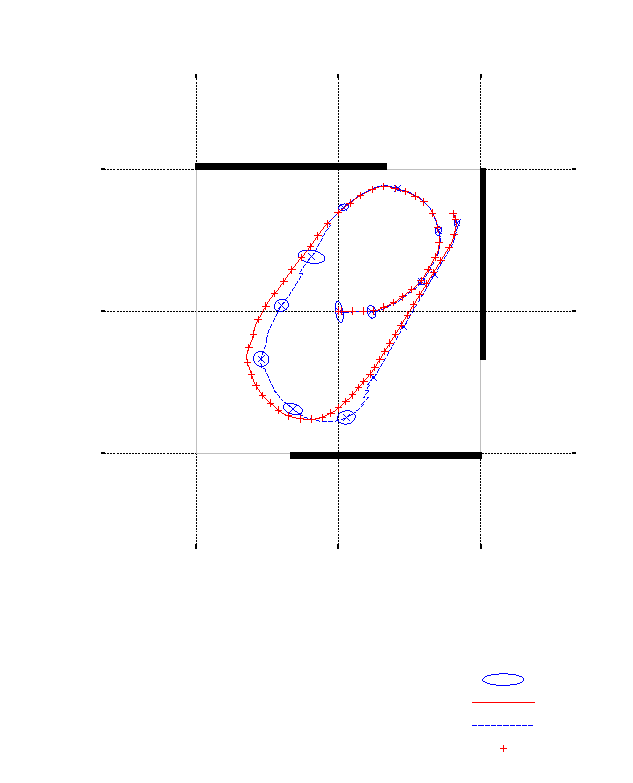
\includegraphics{chapter3/every500mspics_Oval}}%
    \gplfronttext
  \end{picture}%
\endgroup

    \caption{Fahrkurven oben Serpentinen, unten Oval}
    \label{every1500mspics}
\end{figure}
Dazu werden vier verschiedene Fahrkurven eingesetzt. Zu sehen auf den Abbildungen 
\section{Versuche zum Einfluss von Menschen auf der B�hne}
Hier sollen Versuche zeigen, wie stark Menschen auf der B�hne die Lokalisation mit dem hier vorgestellten Verfahren st�ren. Dabei geht es im wesentlichen darum, dass Menschen im Bild stehen, und so die Bit-Muster ganz oder teilweise verdecken.

  

